\documentclass[10pt,uplatex,a4j]{jsarticle}

\usepackage[dvipdfmx]{graphicx}
\usepackage{here}
\usepackage{float}
\usepackage{url}
\usepackage{fancyhdr}

\setlength{\textwidth}{377pt}
\setlength{\oddsidemargin}{37pt}
\setlength{\textheight}{600pt}

\fboxsep=0pt
\fboxrule=1pt

\pagestyle{empty}
\renewcommand{\baselinestretch}{1.0}

\begin{document}


%\setlength{\textwidth}{377pt}
%\setlength{\oddsidemargin}{37pt}
%\setlength{\evensidemargin}{37pt}
\pagestyle{empty}

\begin{titlepage}

\vspace*{1cm}

\begin{center}


修\ \ 士\ \ 論\ \ 文

\vspace*{0.8cm}

題\ 目

\vspace*{1cm}

{\large{カウンターセールスを行うマルチモーダル音声対話システムの構築}}


\vspace*{-0.3cm}

\underline{\hspace*{12cm}}

\vspace*{3cm}

指導教員

\vspace*{0.3cm}

{\large{竹~内~~孔~一}}

\vspace*{-0.3cm}

\underline{\hspace*{4cm}}

\vspace*{3cm}

報~~告~~者

\vspace*{0.3cm}

{\large{山~崎~瑶}}

\vspace*{-0.3cm}

\underline{\hspace*{4cm}}

\vspace*{0.5cm}

岡山大学大学院自然科学研究科電子情報システム工学専攻

\vspace*{2cm}

令和4年2月3日提出





\end{center}
\end{titlepage}
\newpage

% \setlength{\textwidth}{377pt}
% \setlength{\oddsidemargin}{37pt}
% \setlength{\evensidemargin}{37pt}
\pagestyle{empty}

\begin{titlepage}

\vspace*{1cm}

\begin{center}


修\ \ 士\ \ 論\ \ 文

\vspace*{0.8cm}

題\ 目

\vspace*{1cm}

{\large{人型ロボットを用いた対話AIの構築}}

\vspace*{-0.3cm}

\underline{\hspace*{12cm}}

\vspace*{3cm}

指導教員

\vspace*{0.3cm}

{\large{~}}

\vspace*{-0.3cm}

\underline{\hspace*{4cm}}

\vspace*{3cm}

報~~告~~者

\vspace*{0.3cm}

{\large{山~崎~瑶}}

\vspace*{-0.3cm}

\underline{\hspace*{4cm}}

\vspace*{0.5cm}

岡山大学大学院自然科学研究科電子情報システム工学専攻

\vspace*{2cm}

令和4年2月3日提出





\end{center}
\end{titlepage}
\newpage


\thispagestyle{empty}
\section*{要約}
近年,Siriなどのスマートフォン上で動作する音声エージェントやAlexaなどのスマートスピーカに代表されるように
音声対話技術が進展してきている.これは既に社会において音声を通じて対話するシステムが受け入れられて
活用されていると見ることができる.しかしながら,人の日常活動における対話は,上述のスマートスピーカとの
対話よりも複雑であり,現在の音声対話技術でも対話を継続して目的を達成することは困難である.
例えば,カウンターセールス(接客業務)では,対話の内容にに応じて,言葉だけでなく
視線や表情,身振り手振りなどのジェスチャを通じて対話相手の要求に応えていく.
こうした対話における言葉に付随する複数の要素を通じて,実際の人と対話できるシステムは
どのように構築すれば良いかの方針がまだ明らかになっていない.
そこで本研究ではカウンターセールスをタスクを対象とした音声対話システムを構築して
人との対話実験を行うことで構築したシステムの評価を行う.具体的にはセールスの内容として
旅行業務に焦点を置くとともに,対話だけではなく,視線や表情だけでなくジェスチャまで
コントロールできるアンドロイドを活用した音声対話システムを構築する.
評価実験として対話ロボットコンペティションに参加し,ショッピングモール内の雑音がある部屋で
人と対話する実験を行った.動作確認実験と共に対話体験者に対してアンケートによる評価を得たので報告する.



\newpage
\setcounter{tocdepth}{3}
\tableofcontents
\newpage

\pagestyle{fancy}
%\rhead{\leftmark}
%\lhead{\rightmark}
\lhead{\leftmark}
%\rhead{}
\rhead{\thepage}
\lfoot{}
\cfoot{}
\rfoot{岡山大学大学院自然科学研究科\\電子情報システム工学専攻}
\renewcommand{\footrulewidth}{0.4pt}

\setcounter{page}{1}

\section{はじめに}
\label{はじめに}

\subsection{研究背景}
\label{研究背景}
近年,Apple社のSiriなどのスマートフォン上で動作する音声エージェントサービスや,Amazon社のAlexaなどのスマートスピーカーに見られるように,ユーザの発言に対して正しい応答や人間らしい応答を返すための音声対話技術がめざましく進歩している.今後,このような対話システムは,様々な形で,私達の日常活動を支援するものと期待される.\cite{kikiyaku2012} \cite{koreisya2000}しかし,日常活動での対話は,スマートスピーカーとの対話よりも複雑であり,現在の音声対話技術でも,様々な状況においてうまく対話を継続して目的を達成するのは困難である\cite{hitask2016}.例えば対話を通した接客業務では,話し方や要望の出し方など対話相手よって様々であり,それに適切に対応する必要がある.このとき,私達人間であれば,対話相手のタイプによって話し方を切り替えて対応したり,音声だけでなく視線や表情などもうまく使って対話を継続することができるが,音声対話システムではこのような対応を取ることができない.人型ロボットは,様々なセンサを用いてユーザの音声だけでなく表情やしぐさなどを認識できたり,体を用いてジェスチャや表情など様々な表現ができる.音声対話システムよりも複雑である反面,多くの情報や多くの表現手段を用いることで,従来の対話システムとは異なる方法で対話をうまく継続を実現できる可能性がある.本研究では音声,表情,身振り,手振りなどのモダリティを用いて円滑に対話を進めるマルチモーダル音声対話システムの構築を目指す.

\subsection{研究の位置付け}
情報化社会の次に来るであろう人間と知能ロボットや情報メディアが共生する社会を実現するため,「人間機械共生社会を目指した対話知能システム学(対話知能学)」\footnote{https://www.commu-ai.org/}が文部科学省科学研究費助成事業「新学術領域研究」として2019年に創生された.対話内容を完全に理解できずとも違和感なく対話を継続できる能力を実現する「対話継続関係維持」,特定の状況において特定の目的に関して対話理解と対話生成を組み合わせた対話能力を実現する「対話理解生成」,システムが自らの行動決定モデルを構築したり相手の行動決定モデルを推定する機能を実現する「行動決定モデル推定」,実証実験を通して意図や欲求を持つロボットの人々への影響を研究,ロボット共生社会における社会規範を提案する「人間機械社会規範」の4つの軸を元に,人間と機械や情報メディアが互いの意図や欲求を推定し合いながら関わり合う社会の実現を目指す.複数の情報を統合し状況に適応的にふるまうマルチモーダル音声対話システムの構築は「対話理解生成」に相当する.
\begin{figure}[th]
    \centering
    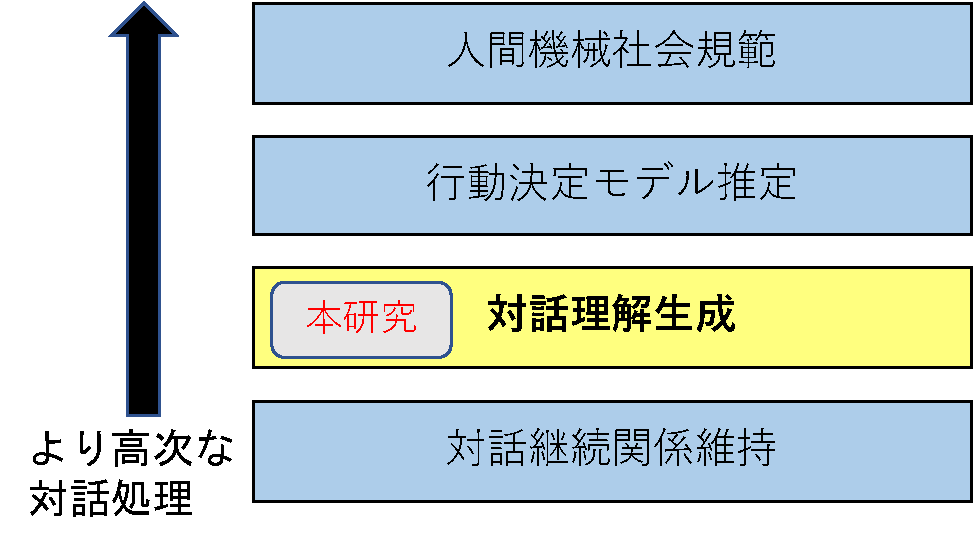
\includegraphics[scale=0.5]{pic/commuai.pdf}
    \caption{対話システム構築の位置付け}
    \label{commuai}
\end{figure}


\subsection{研究目的}
\label{研究目的}
本研究では,旅行代理店業務において,カウンターセールスを行う音声対話システムの構築を目指す.対話システムは,音声,表情,身振り,手振りなどのモダリティをもち,身体性も有する.複数のモジュールを用いてロボットの身体管理,対話管理を行うことでロボットと音声で対話実現をすることで,テキストだけの対話システムや音声だけの対話システムに比べ,ホスピタリティの高い対話を実現することを目標とする.

\subsection{本論文の構成}
\label{本論文の構成}
以下に本論文の構成を記述する.\ref{関連研究}章では,音声対話システムの関連研究について説明する. \ref{対話システムの構築}章では提案手法の概要とシステムのモジュールについて説明する.\ref{評価実験}章では対話ロボットコンペティションにおいての実験について述べる.\ref{考察}章で構築した対話システムに関する考察を行い,\ref{まとめ}章でまとめについて述べる.

\section{関連研究}
\label{関連研究}
本章では,音声対話システムに関する先行研究について述べる.

\subsection{音声対話システムに関する先行研究}
\label{音声対話システムに関する先行研究}

対話システムは,数度のフェーズを経て,古いものでは1950年代後半から開発が行われている.\cite{higashinaka2020python}初期の対話システムとしてWeizenbaumのELIZA\cite{weizenbaum1966eliza}やWinogradのSHRDLU\cite{winograd1971shrdlu}が挙げられる.ELIZAは手作業で作成したIf-Thenルールに基づき挙動するシステムで,簡単な単語の一致によるパターンマッチングにより動作する.SHRDLUは対話により積み木を動かすというシステムで,「赤いブロックを左に移動して」という発言に対し,赤いブロックが2つある場合「どちらの赤いブロックですか?」等の問い返しをすることができる.これらの2つのシステムは限定的な状況でしか問題を解決することができず,現実の問題を解決するには至っていない.1980年代になると,データベースをもとにしたエキスパートシステムが台頭する.BuchananらのMYCIN\cite{buchanan1984rule}は医療診断システムとして専門医に若干劣るほどの診断を可能とした.BobrowらのGUS\cite{bobrow1977gus}はフレーム表現と呼ばれる知識構造を利用し,ユーザの発話から発話理解を行う.フレーム表現は今日の対話システムでも利用されることが多く,本実験でもフレーム表現を利用して構築を行う.エキスパートシステムのデータベース作成は全て手作業で行われるため,専門知識を体系的にシステムに落とし込む作業がボトルネックとなった.2000年代になると機械学習の発展により,事例から対話を生成することが可能となる.WuらのTOD-BERT\cite{wu2020tod}は10万件を超える対話事例から対話を自動生成する.機械学習により音声認識や音声合成などの精度も飛躍的に向上し,音声認識や音声合成を用いた対話システムの構築が積極的に行われている.\cite{higsshinakalive}

\subsection{対話システムの類型}
\label{対話システムの類型}
対話システムは以下のような観点で分類することができる.
\begin{description}
    \item[タスクの有無]
    \item[ユーザの人数]
    \item[モダリティ]
    \item[主導権]
    \item[身体性の有無]   
\end{description}

\section{対話システムの構築}
\label{対話システムの構築}
%\subsection{対話システムの全体像}
本章では,対話システムの構築方法について述べる.対話システムは,ロボットのハードウェアを制御するロボット管理と対話の制御を行う対話管理に分けることができる.対話システムの全体像を図\ref{overview_system}に示す.ロボット管理と対話管理の通信は全てTCPで行う.ロボット管理の各モジュールではそれぞれの部位に対応するロボットの制御を行う.\ref{対話システムを構成するモジュール}節で各モジュールの詳しい説明を行う.対話管理ではユーザの発話を理解し,システムの発話や行為を決定する.\ref{対話管理}節で対話管理について詳しく述べる.

\begin{figure}[th]
    \centering
    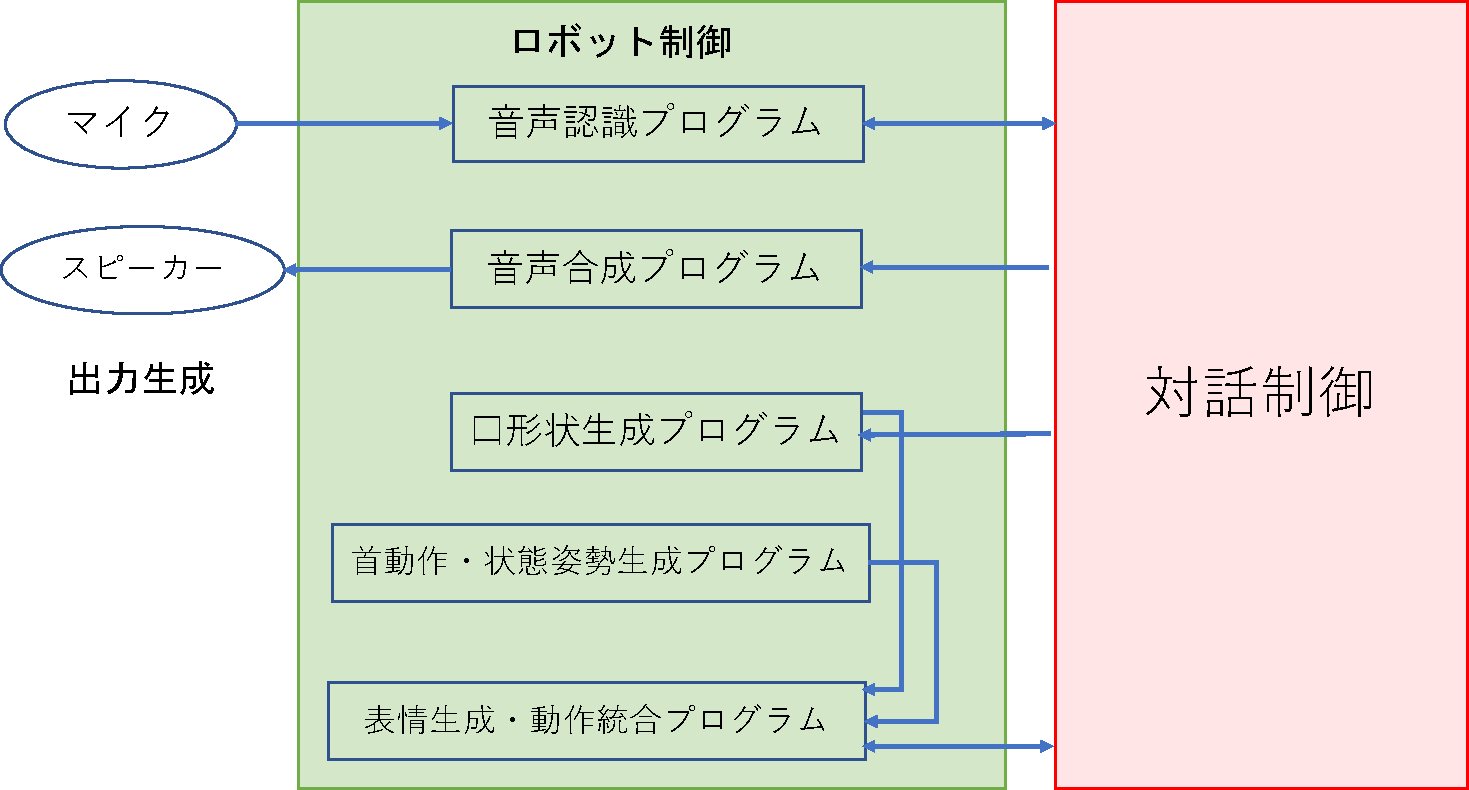
\includegraphics[scale=0.5]{pic/overview_system.pdf}
    \caption{対話システムの全体像}
    \label{overview_system}
\end{figure}

\subsection{ロボット管理}
\label{対話システムを構成するモジュール}
対話ロボットとして,国際電気通信基礎技術研究所(ATR)\footnote{https://www.atr.jp/}が管理するアンドロイドを使用する.身長165センチ,体重38キログラムであり,空気圧アクチュエータで駆動する.本節でロボットを制御するモジュールを詳しく述べる.
\begin{figure}[th]
    \centering
    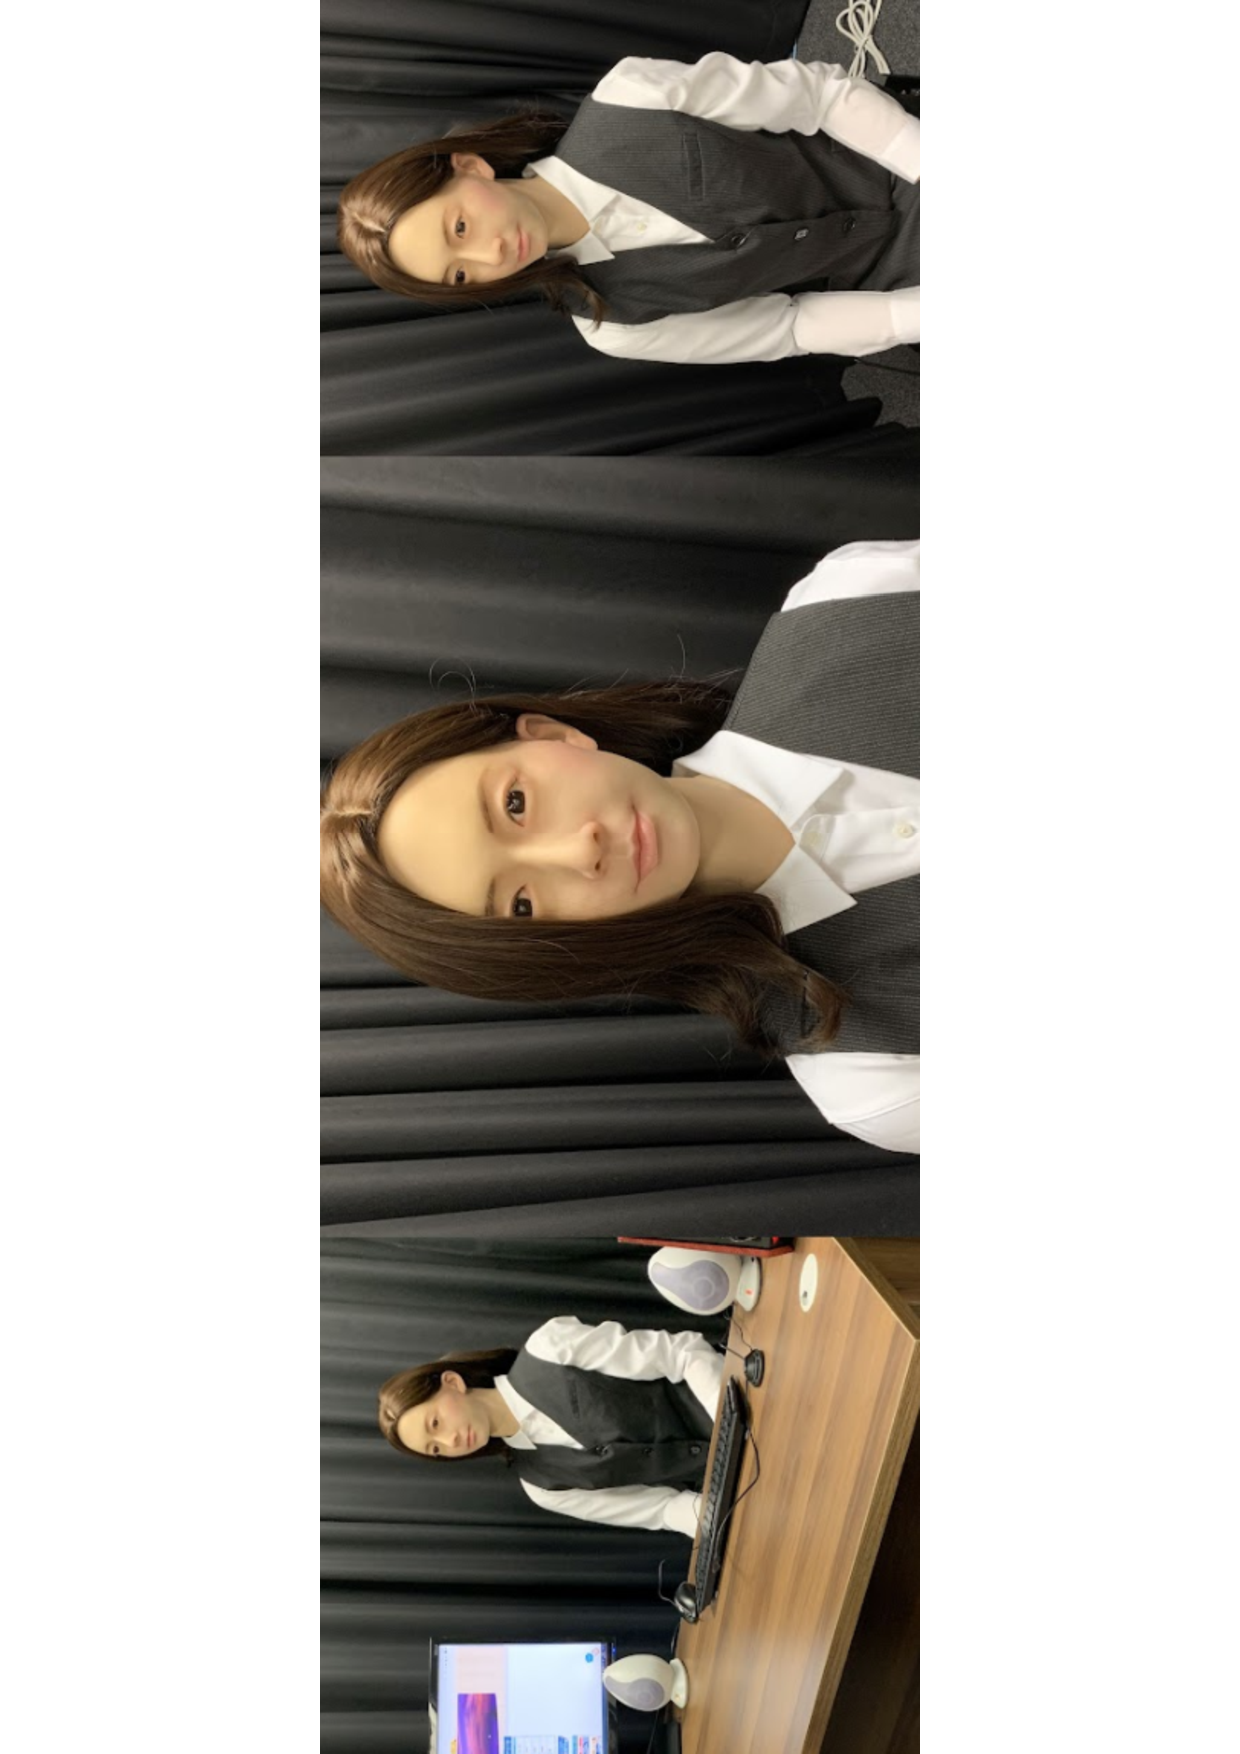
\includegraphics[scale=0.4,angle=270]{pic/ai.pdf}
    \caption{アンドロイドの近景}
    \label{kinkei}
\end{figure}

\subsubsection{音声認識}
音声認識にはGoogleのSpeech-to-Textを利用する.文字コードはutf-8で,音声認識を開始してからマイク入力があると,途中結果を返しながら最終結果と信頼度を返すストリーミング形式の通信を行う.コマンドのフッターは改行コードである.送信プロトコル,受信プロトコルを表\ref{sendrecv}に示す.

\begin{table}[hbtp]
    \caption{送受信プロトコル}
    \label{sendrecv}
    \centering
    \begin{tabular}{l|l}
    \hline
    送信プロトコル                         & 受信プロトコル                  \\ \hline
    音声認識スタート start\textbackslash{}n & 音声認識スタート startrecog:      \\
    音声認識ストップ stop\textbackslash{}n  & 音声認識途中結果 interimresult:  \\
                                    & 音声認識最終結果 result:          \\ 
                                    &  最終結果の信頼度 confidence:       \\ \hline
    \end{tabular}
\end{table}

1度音声認識を開始すると音声認識を終了するまでずっと音声認識をする.受信サンプルを時系列順に並べると以下のようになる.
\begin{table}[hbtp]
    \centering
    \begin{tabular}{|l|}
    \hline
    startrecog:\\
    interimresult:今日\\
    interimresult:今日は\\
    interimresult:今日は\\
    interimresult:今日は週\\
    interimresult:今日は中止\\
    interimresult:今日は中止度\\
    interimresult:今日は修士論文\\
    nterimresult:今日は修士論文発\\
    interimresult:今日は修士論文発表\\
    interimresult:今日は修士論文発表会です\\
    result:今日は修士論文発表会です\\
    confidence:0.9313719153404236\\
    \hline
    \end{tabular}
\end{table}

\subsubsection{音声合成}
音声合成にはAmazonのAmazon Pollyを使用した.通信方式は同期通信で,全てJSON形式でやりとりが行われる.文字コードはutf-8で,コマンドのフッターは改行コードである.再生に成功した場合,
\begin{table}[hbtp]
    \centering
    \begin{tabular}{l}
    \{(送信)再生コマンド $\rightarrow$\\ 
    (受信) \{"result":"success-start","duration":12491\} \\
    $\rightarrow$ (受信)\{"result":"success-end"\}\\
    \end{tabular}
\end{table}    
のように,音声の再生開始,終了と音声の再生時間を受信する.失敗した場合は,
\begin{table}[hbtp]
    \centering
    \begin{tabular}{l}
    \{(送信)再生コマンド $\rightarrow$ (受信)\{"result":"failed"\}
    \end{tabular}
\end{table}
となる.また,

\begin{table}[hbtp]
    \centering
    \begin{tabular}{l}
        (送信)\{"engine":"ISSPEAKING"\} $\rightarrow$(受信)\{"isSpeaking":true/false\}
    \end{tabular}
\end{table}

で現在発話中かを確認することができ,

\begin{table}[hbtp]
    \centering
    \begin{tabular}{l}
        (送信)\{"engine":"STOP"\} $\rightarrow$ (受信)\{"result":"success-end"\}
    \end{tabular}
\end{table}

で再生中に音声を停止することができる.
音声合成に使用するパラメータを表に示す.


システムに標準のピッチ,声量,大きさで「コマンドサンプル」と発話させるためのコマンドの例を以下に示す.
\begin{table}[hbtp]
    \centering
    \begin{tabular}{c}
        \{"engine":"POLLY", "speaker": "Mizuki",  "pitch": 100, "volume":100, \\
        "speed":100,"vocal-tract-length":0, "duration-information":false,  \\
        "speechmark":false, "text":"コマンドサンプル"\}\textbackslash{}n
    \end{tabular}
\end{table}


\subsubsection{口形状生成}
口形状生成には,OculusのOculus Lipsync Unityを利用する.Oculus Lipsync Unityはマイク入力やオーディオファイルからのオーディオインプットストリームを分析し,口形素と呼ばれる唇や顔の表情の一連の値を予測するソフトウェアである.プログラムにアクセスする必要はなく,合成音声を再生すると,それに同期するようにアンドロイドの口形状を制御する.

\subsubsection{首動作・状態姿勢生成}
%MiracleHuman
首動作・状態姿勢生成は非同期通信で行い,コマンドのフッターは改行コード,文字コードはutf-8である.視線,上体姿勢,感情状態を任意の タイミングで指令することができる.ロボットの正面方向をz軸,右をx軸,上をy軸,ロボットの腰の下を原点とした座標系で,x,y,zで視線,顔,体を向ける座標をメートル単位で指定することができる.ロボットの視線を,正面の1.5メートル先,高さ1.2メートルの位置に向ける際のコマンドを以下に示す."translateSpeed"で表される移動速度の単位はメートル毎秒である.
\begin{table}[hbtp]
    \centering
    \begin{tabular}{l}
        EyeController=\{"id": "EyeController","motionTowardObject": "",\\
        "targetMotionMode": 2,"targetPoint": \{"x": 0.0,"y": 1.2,"z": 1.5\},\\
        "translateSpeed": 2.0\}\textbackslash{}n
    \end{tabular}
\end{table}
また,座標指定で動作をせず,事前に定義されたジェスチャを指示することもできる.定義されたジェスチャでは両手の指の開閉や,頭のみ,首のみ,全身を使ったお辞儀,首や視線の縦振り,横振りを指示することができる.

\subsubsection{表情生成・動作統合}
%JointMapperPlusUltraSuperFace
表情生成・対話生成は非同期通信で行い,コマンドのフッターは改行コード,文字コードはutf-8である.事前に定義された表情のラベルにより,頬,口角,眉毛などの位置を制御し,表情を変化させる.表情のラベルを図\ref{labels}に示す.瞬きは支持する必要がなく,定感覚で自動で行われる.

\begin{table}[hbtp]
    \caption{定義された表情ラベル}
    \label{labels}
    \centering
    \begin{tabular}{l|l}
    \hline
    表情名           & 説明              \\ \hline
    MoodBasedFACE   & 基本の表情           \\
    fullsumile      & 笑ったような表情        \\
    angry           & 怒ったような表情        \\
    bad             & 印象の良くない表情       \\
    mouth-a/i/u/e/o & それぞれの母音を発する時の表情 \\ \hline
    \end{tabular}
\end{table}

\subsection{対話管理}
\label{対話管理}
対話管理では,音声認識した発話を文字列で受け取り,発話理解をし,対話のフローとフレーム表現を含めた内部状態の更新,参照を繰り返しながら行動選択,発話生成を行う.本研究で構築する対話システムは「旅行先の決定」というゴールを持ったタスク指向型対話システムである.対話管理で構成する対話の全体の流れを図\ref{flow}に示し,本システムの想定する対話の流れを詳しく述べる.

\begin{figure}[th]
    \centering
    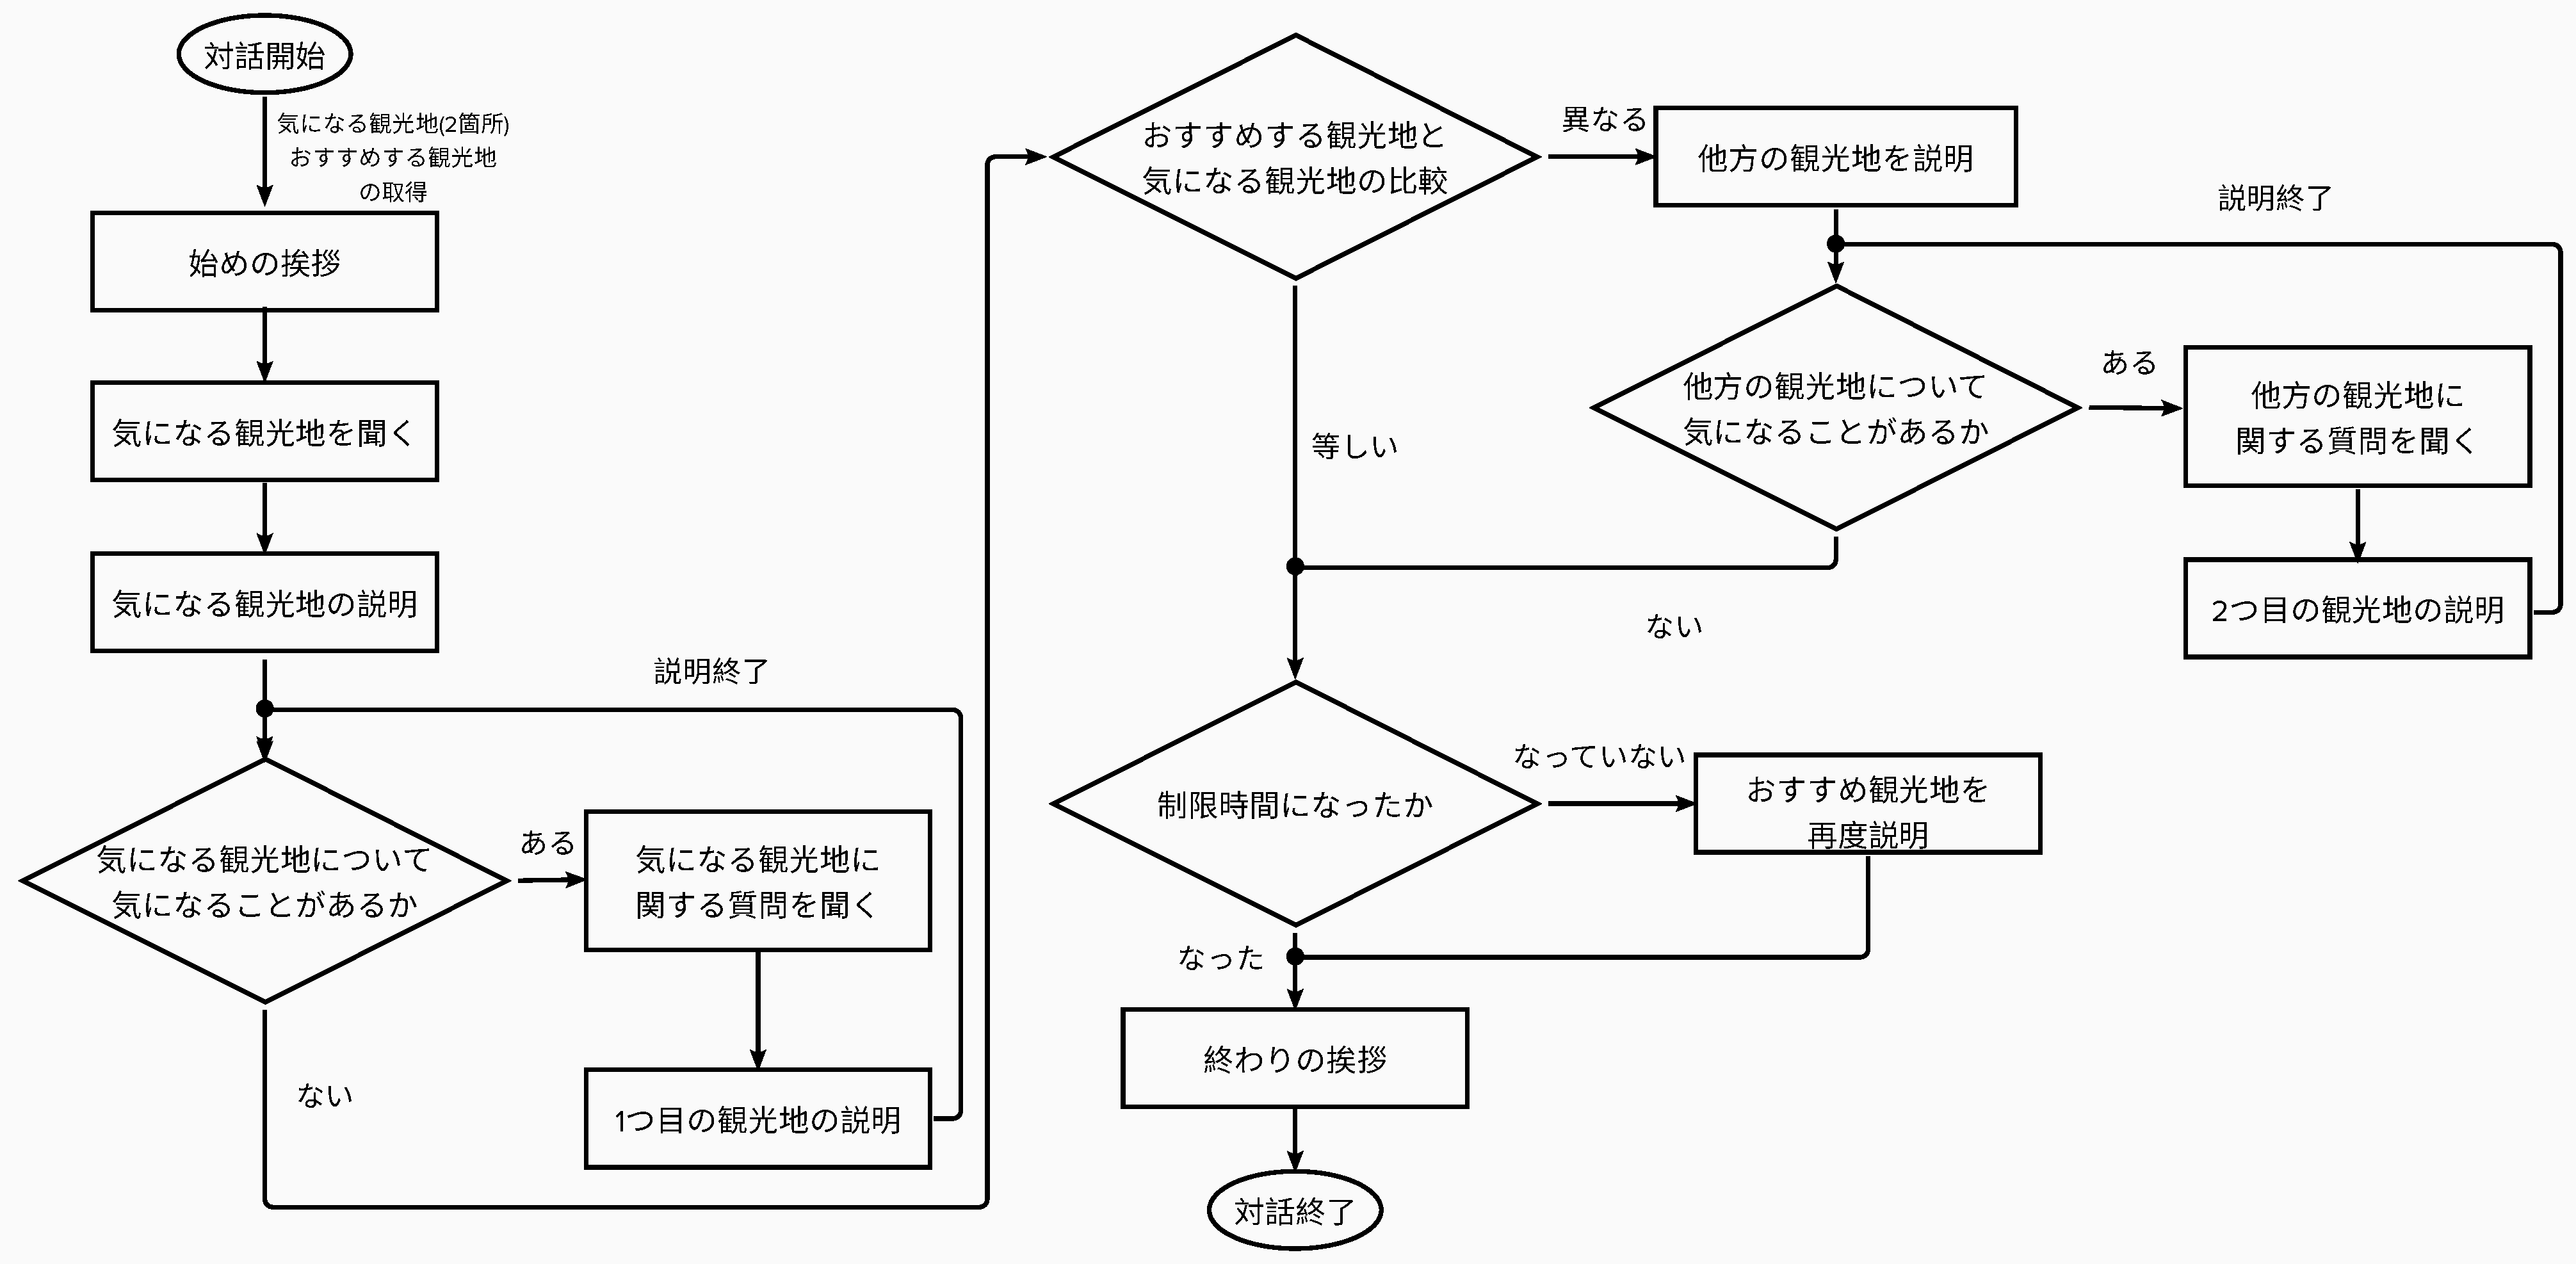
\includegraphics[scale=0.25]{pic/flow.pdf}
    \caption{対話の流れ}
    \label{flow}
\end{figure}

\begin{enumerate}
    \item 対話開始\\
            対話を開始すると,事前にID管理サーバへアクセスし,対話者の選択した2つの観光地と,おすすめ観光地(体験者に選ばせればコンペティションの評価の上がる運営がランダムに選定した勧めるべき観光地.)を取得する.選択した観光地についてどちらの観光地が気になるかを尋ね,気になる観光地の基本情報を説明する.
            \begin{figure}[th]
                \centering
                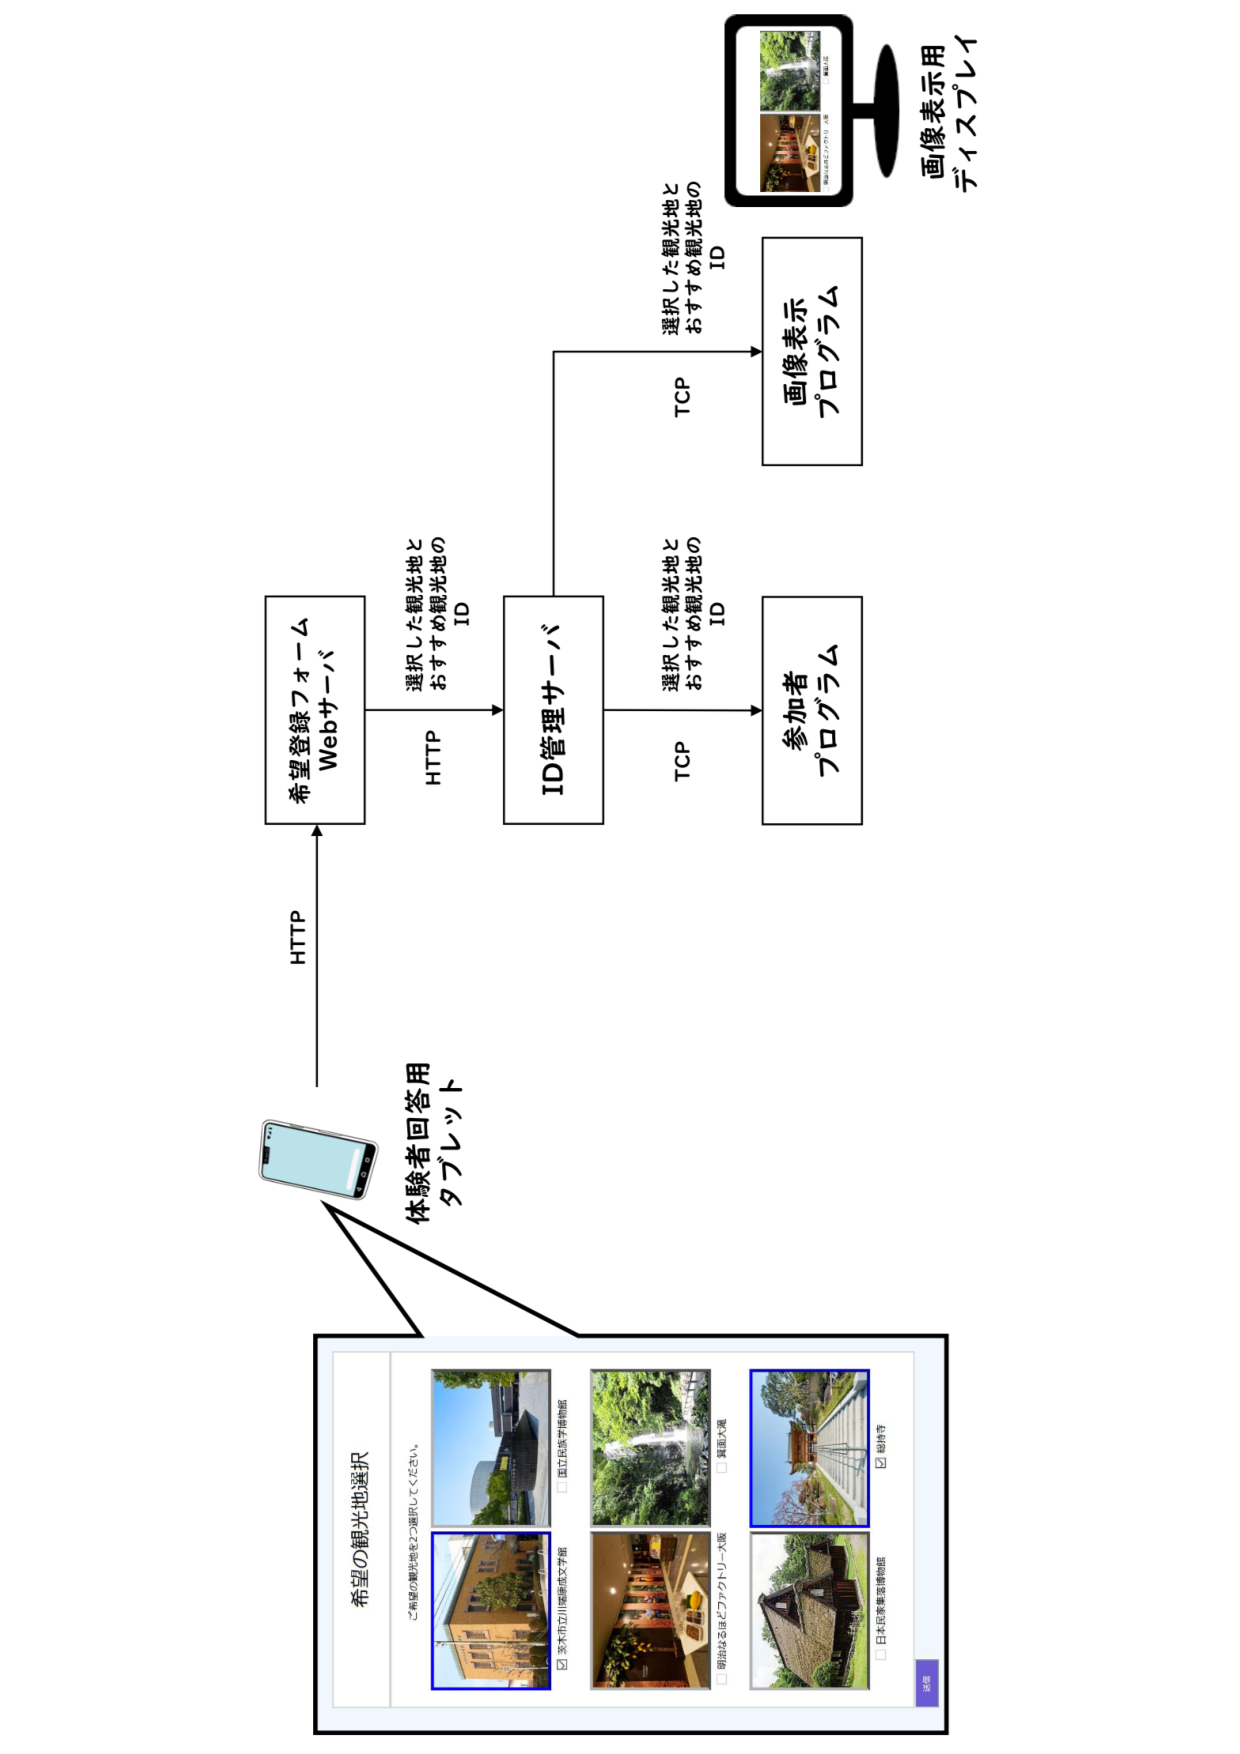
\includegraphics[scale=0.4,angle=270]{pic/how2choice.pdf}
                \caption{観光地の選択システム}
            \end{figure}

    \item 気になる観光地に関する質疑応答\\
            基本情報の説明ののち,「観光地に関して何か気になることはないか」と尋ね,質問がなくなるまで対話者主導で複数回の質疑応答を行う.

    \item 気になる観光地とおすすめ観光地の比較\\
            質問がない場合,気になる観光地とおすすめ観光地の比較を行う.気になる観光地とおすすめ観光地が等しい場合,他方の観光地の説明は行わず,再度気になる観光地についての簡単な説明を行い対話を終了する.気になる観光地とおすすめ観光地が異なる場合は他方の観光地の基本情報を追加で説明する.

    \item 他方の観光地に関する質疑応答\\
            基本情報の説明ののち,「観光地に関して何か気になることはないか」と尋ね,質問がなくなるまで対話者主導で複数回の質疑応答を行う.

    \item 対話終了\\
            他方の観光地について質問が無くなった場合,対話の終了フェーズに入る.定められた対話時間がまだ残っている場合,再度気になる観光地についての簡単な説明を行い対話を終了する.対話時間が来た際は質疑応答の途中でも終わりの挨拶をして対話を終了する.
 \end{enumerate}

 \subsection{言語理解}
 言語理解では対話者の発言から対話行為を推定する.推定には単純な文字列マッチングを用いる.MeCabを用いた形態素解析を行い,ユーザの発言と対話行為タイプの一致判定により対話行為タイプを決める.

\subsubsection{フレーム表現を用いた発話理解}
本システムは「フレーム」と呼ばれるデータ構造を用いて対話を進める.図\ref{frame}に示すように,対話者が事前に選択した2つの観光地,おすすめする観光地,現在話題になっている観光地,対話履歴(観光地とその観光地の何について対話したかの組)を保持する.この例では,現在箕面大滝について話しており,すでに観光地の説明,アクセス方法,車での行き方,駐車場について対話が行われたことがわかる.このようなフレーム表現を用いることで「どのようにすれば行けますか?」という質問に対して,現在話題に上がっている箕面大滝への行き方を尋ねられたとして発話の理解を行うことができる.話題が国立民族学博物館は話題の項目を国立民族学博物館へと変更し対話を進める.この時,「どのようにすれば行けますか?」と同じ質問をされても,話題に上がっている国立民族学博物館への行き方を尋ねられたと理解することができるため,適切な返答をすることができる.

\begin{figure}[th]
    \centering
    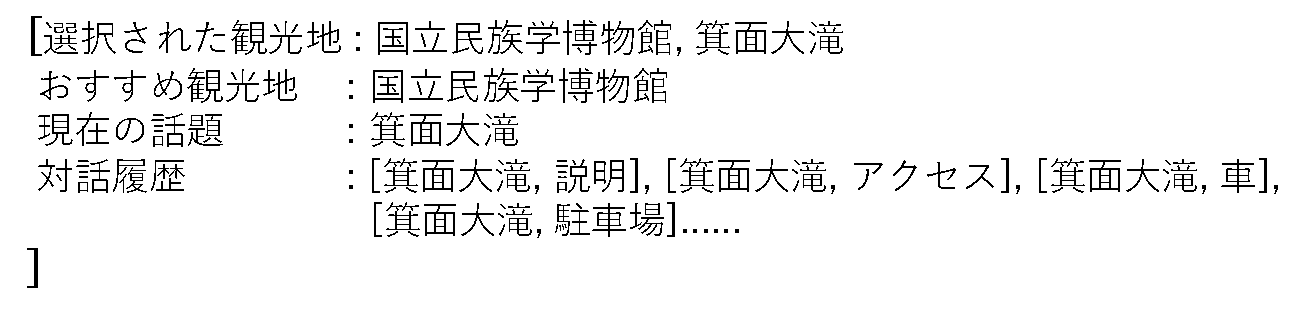
\includegraphics[scale=0.5]{pic/frame.pdf}
    \caption{フレーム表現の例}
    \label{frame}
\end{figure}

私たちは対話の中で主語の省略や指示代名詞をよく使う.例えば,「私は箕面大滝へ行きたいです.そこへはどうやっていきますか.駐車場はありますか.」という文書の場合,「そこ」は直前に述べたを指し,駐車場はありますかという文書には箕面大滝にという語が隠れている.人間はその場の状況を参照し文書の理解を試みるが,システムがなんの情報もなくこの文書を理解することは難しい.このような照応表現の解析は自然言語処理における重要な課題として挙げられ\cite{shouo1996},対話システムの構築においても対話の中での照応解析は大きな問題である\cite{taiwashouo2003}.フレーム表現を利用することで,旅行代理店におけるカウンターセールスという限られた条件の中で,照応解析を実現し,主語の省略や代名詞の使用に対応した人間らしい会話の実現を可能にする.

\subsubsection{行動選択}
内部状態を参照しながら発話理解を行ったのち,行動選択に移る.

\begin{table}[htb]
    \caption{発話行為タイプ}
    \label{sendrecv}
    \centering
    \begin{tabular}{l|l||l|l}
    \hline
    発話行為タイプ     & 説明        & 発話行為タイプ  & 説明\\\hline
    explanation & 概要の説明      & parking  & 駐車場の有無\\
    address     & 住所         & child    & 子供も楽しめるか\\
    time        & 営業時間       & near     & 近隣の飲食店情報\\
    open        & 営業開始時間     & event    & 直近のイベント情報\\
    close       & 営業終了時間     & covid    & covid-19情報\\
    close\_day  & 定休日        & thanks   & お礼\\
    tell        & 電話番号       & yes      & はいと言われた時\\
    accsess     & どうやっていくか   & no       & いいえと言われた時\\
    by\_train   & 電車でのアクセス方法 & stay     & 観光地を迷ってる時 \\
    by\_car     & 車でのアクセス方法  & decision & 観光地を決める時\\
    photo       & 写真撮影の可否    & error    & 対話理解ができなかった時\\
    height      & 観光地の高さ     & benefit  & ご利益(総持寺)\\
    width       & 観光地の広さ    & goshuin  & 御朱印(総持寺)\\
    seasons     & 訪問におすすめの季節 & swim     & 遊泳の可否(箕面大滝)\\ 
    tourists    & 年間観光客数     & choco    & チョコレートの飲食\\
    price       & 発生する料金 & &(明治なるほどファクトリー大阪) \\
\hline
    \end{tabular}   
\end{table}



\subsection{対話を円滑に進める機構}
\subsubsection{対話破綻の抑止}
対話システムがユーザに対して不適切な返答をしてしまう「対話破綻」と呼ばれる現象が起こることがある.対話破綻は大きく4つに分類することができる\cite{challenge2015}.

\begin{enumerate}
    \item 構文などの崩れにより,日本語として成立せず発話そのものが破綻している場合
    \item 日本語としては正しいが,相手の発言に対する「応答」として成立せず破綻している場合
    \item 単発のやりとりとしては成立しているが、既に話した内容と異なる発話をするため,「文脈」が破綻している場合
    \item 社会通念や倫理的におかしな発言をしてしまう場合
\end{enumerate}

体験者の発話から,返答を生成して応答せず,あらかじめ用意された返答を返すため,1つめと4つめの対話破綻は未然に防ぐことができる.また,フレーム表現を用いて対話履歴を参照しながら対話を進めるため,発話の整合性を保ちながら対話を進め,3つめの対話破綻を防ぎながら対話を進める.

2つめの,日本語としては正しいが,相手の発言に対する「応答」として成立せず破綻している場合の典型的な例として,音声認識や発話認識,行動選択をしている間に対話者が新たな発話を行うことで,発話認識,行動選択を再度開始してしまうといったケースが挙げられる.この場合,システムは発話すべきテキストを複数抱えてしまい,円滑に対話が進まなくなる.発話内容とアンドロイドの姿勢・表情の2つの面からこの破綻を防ぐ.

\begin{description}
    \item[発話内容]
    システムが発話を終了する際は全て疑問文で終わる.システムの発言する順番と対話者が発言する順番を明確にすることで,発話認識,行動選択をしている間に対話者が新たな発言をすることを防ぐことができる.
    \item[アンドロイドの姿勢・表情]
    システムが発話を終了した際と音声認識を完了した際に笑顔で頷く.対話者にシステムの発話が終了したことや,音声が正常に認識されたことを表情により示すことで,対話者が不要な発言をすることを防ぐことができる.
\end{description}

\subsubsection{観光地に関する情報の拡充}
6箇所の観光地に関する基本情報として,運営から,るるぶDATA\footnote{旅行ガイドブック「るるぶ情報版」掲載の観光情報コンテンツのデータベース.} \footnote{https://solution.jtbpublishing.co.jp/service/domestic/}を使用した観光案内情報を付与されたが,情報量が不十分であったため,Google Maps APIと手作業による観光地情報の拡充を行なう.

事前にGoogle Maps APIにより観光地周辺の飲食店について情報を収集し,データベースを作成することで,観光地の周辺情報について聞かれた際の返答を用意した.また,「箕面大滝で遊泳することは可能か」,「明治なるほどファクトリーでチョコレートを試食することは可能か」など,各観光地に対して事前に想定される質問への回答を手作業でいくつか用意することで対話の成功確率の向上を試みた.

\section{評価実験}
\label{評価実験}

本章では\ref{対話システムの構築}章で説明した対話システムの評価について説明する.対話システムの評価する枠組として,
大阪府吹田市にある大型複合施設EXPOCITY内にあるショッピングモール「ららぽーとEXPOCITY」で実施された
対話ロボットコンペティション\footnote{https://sites.google.com/view/crobotcompetition}を利用する.
対話ロボットコンペティションは複数の対話研究チームを公募し,下記のように規定された旅行代理店業務を対話ロボット
に実施させることによって対話を実施し,その評価を行う.下記に詳細を記述する.

\subsection{実験設定}

\subsubsection{旅行代理店対話タスク}
対話ロボットコンペティションでは,旅行代理店における対話タスクとして,カウンターセールス役となったロボットが,対話を通してお客様役である対話者の要望に応える.体験者は図\label{6place}に示す通り,「日本民家集落博物館」,「茨木市立川端康成文学館」,「総持寺」,「日本民家集落博物館」,「箕面大滝」,「明治なるほどファクトリー大阪」の6箇所の観光地候補から行きたい2箇所決め,そのどちらに行きたいをシステムとの対話を通して決める.
\begin{figure}[th]
    \centering
    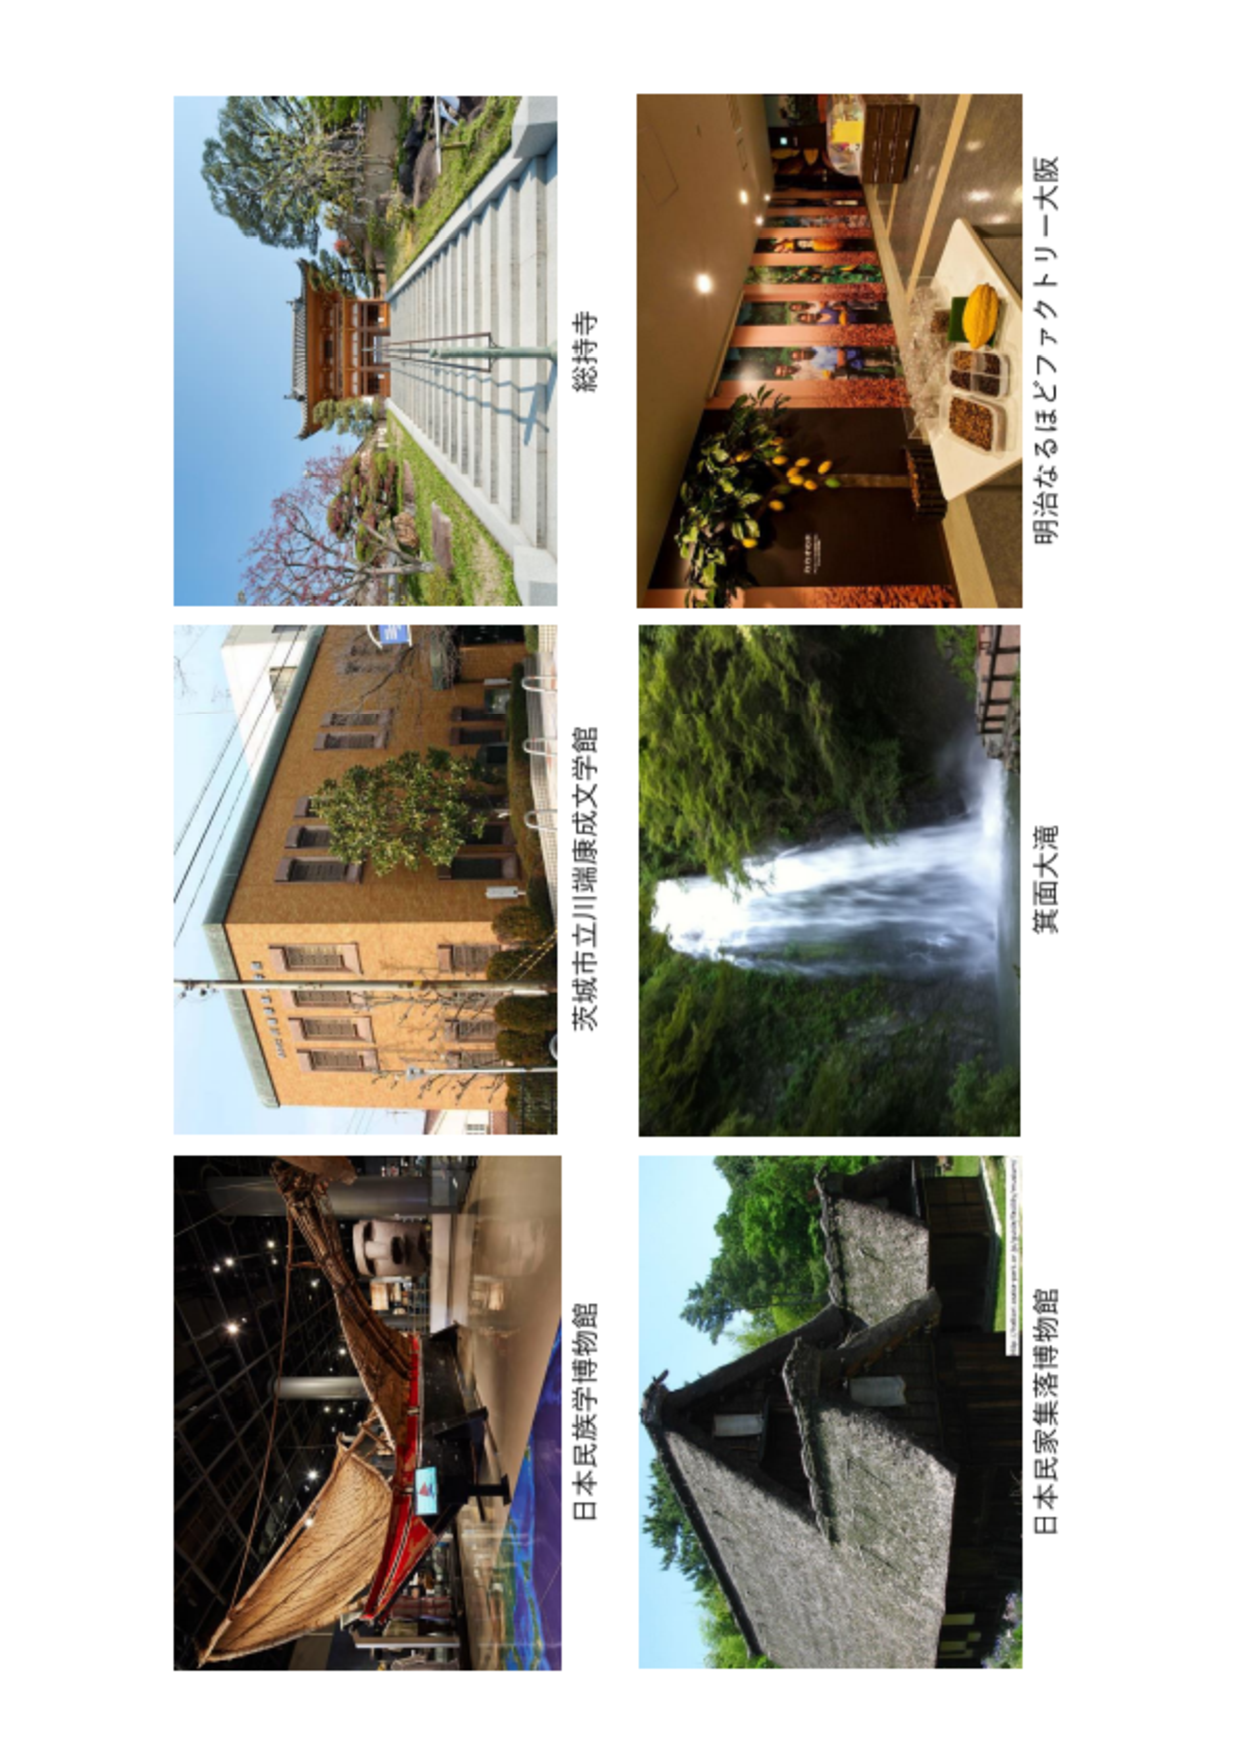
\includegraphics[scale=0.5,angle=270]{pic/6place.pdf}
    \caption{観光地の候補}
    \label{6place}
\end{figure}

\subsubsection{体験やへの事前の指示}
ロボットと対話する体験者は,当日「ららぽーとEXPOCITY」を訪れた買い物客であるため,実際に対話をするにあたり,以下のような事前の指示を行う.

\begin{itemize}
    \item 日本語でロボットと対話して頂きます.
    \item お客様役として振る舞って頂きます.
    \begin{itemize}
        \item Expo Cityに休暇で訪れる予定を持っており,その近辺で1日遊びに行く観光地を決める目的を持っているつもりになって,カウンターセールス役のロボットに相談してください.
        \item 対話を行う前に,近辺の観光地候補の中から行ってみたいと思う観光地を2箇所選んでください.カウンターセールス役のロボットと相談して,体験者自身がお金を払ってでも遊びに行きたいと思える観光地をその2箇所の中から1箇所を決めてください.
        \item 2つの観光地に関する情報をまんべんなく確認して,行きたい観光地を決めてください.
    \end{itemize}
    \item 対話中の注意事項
    \begin{itemize}
    \item カウンターの椅子に座ってから対話を始めてください.
    \item ロボットと相談する時間は最大5分間です.5分経過すると対話を終えて頂きます.5分経過する前に行きたい場所が決まった場合は,カウンター上のタブレットの「行きたい場所を決めた」ボタンにタッチして対話を終えてください.
    \item 相談が終わった後,カウンター上のタブレット上に,ただいまの対話についての質問が表示されますので,それについて回答して頂いた後,行きたい観光地(強いて行きたいならどこか)を選んでください(対話を通して観光地の情報がうまく聞き出せなかった場合などで選ぶのが難しい場合は「選べない」を選択して頂くことも可能です).
    \item 最後に,体験についてのアンケートについてタブレットで回答して頂きます.
    \end{itemize}
\end{itemize}

\subsubsection{レギュレーション}
対話ロボットコンペティションではレギュレーションが定められており,このレギュレーションに従って開発,実装を行なう.
\begin{enumerate}
    \item 対話状況
    \begin{itemize}
        \item 体験者とロボットは1対1で対話する.
        \item カウンターテーブルの大きさ,ロボットと体験者の椅子の位置は固定.
        \item テーブル上に体験者とロボットが同時に見ることができるようにモニタを設置(位置と向きは固定).
    \end{itemize}
    \begin{figure}[th]
        \centering
        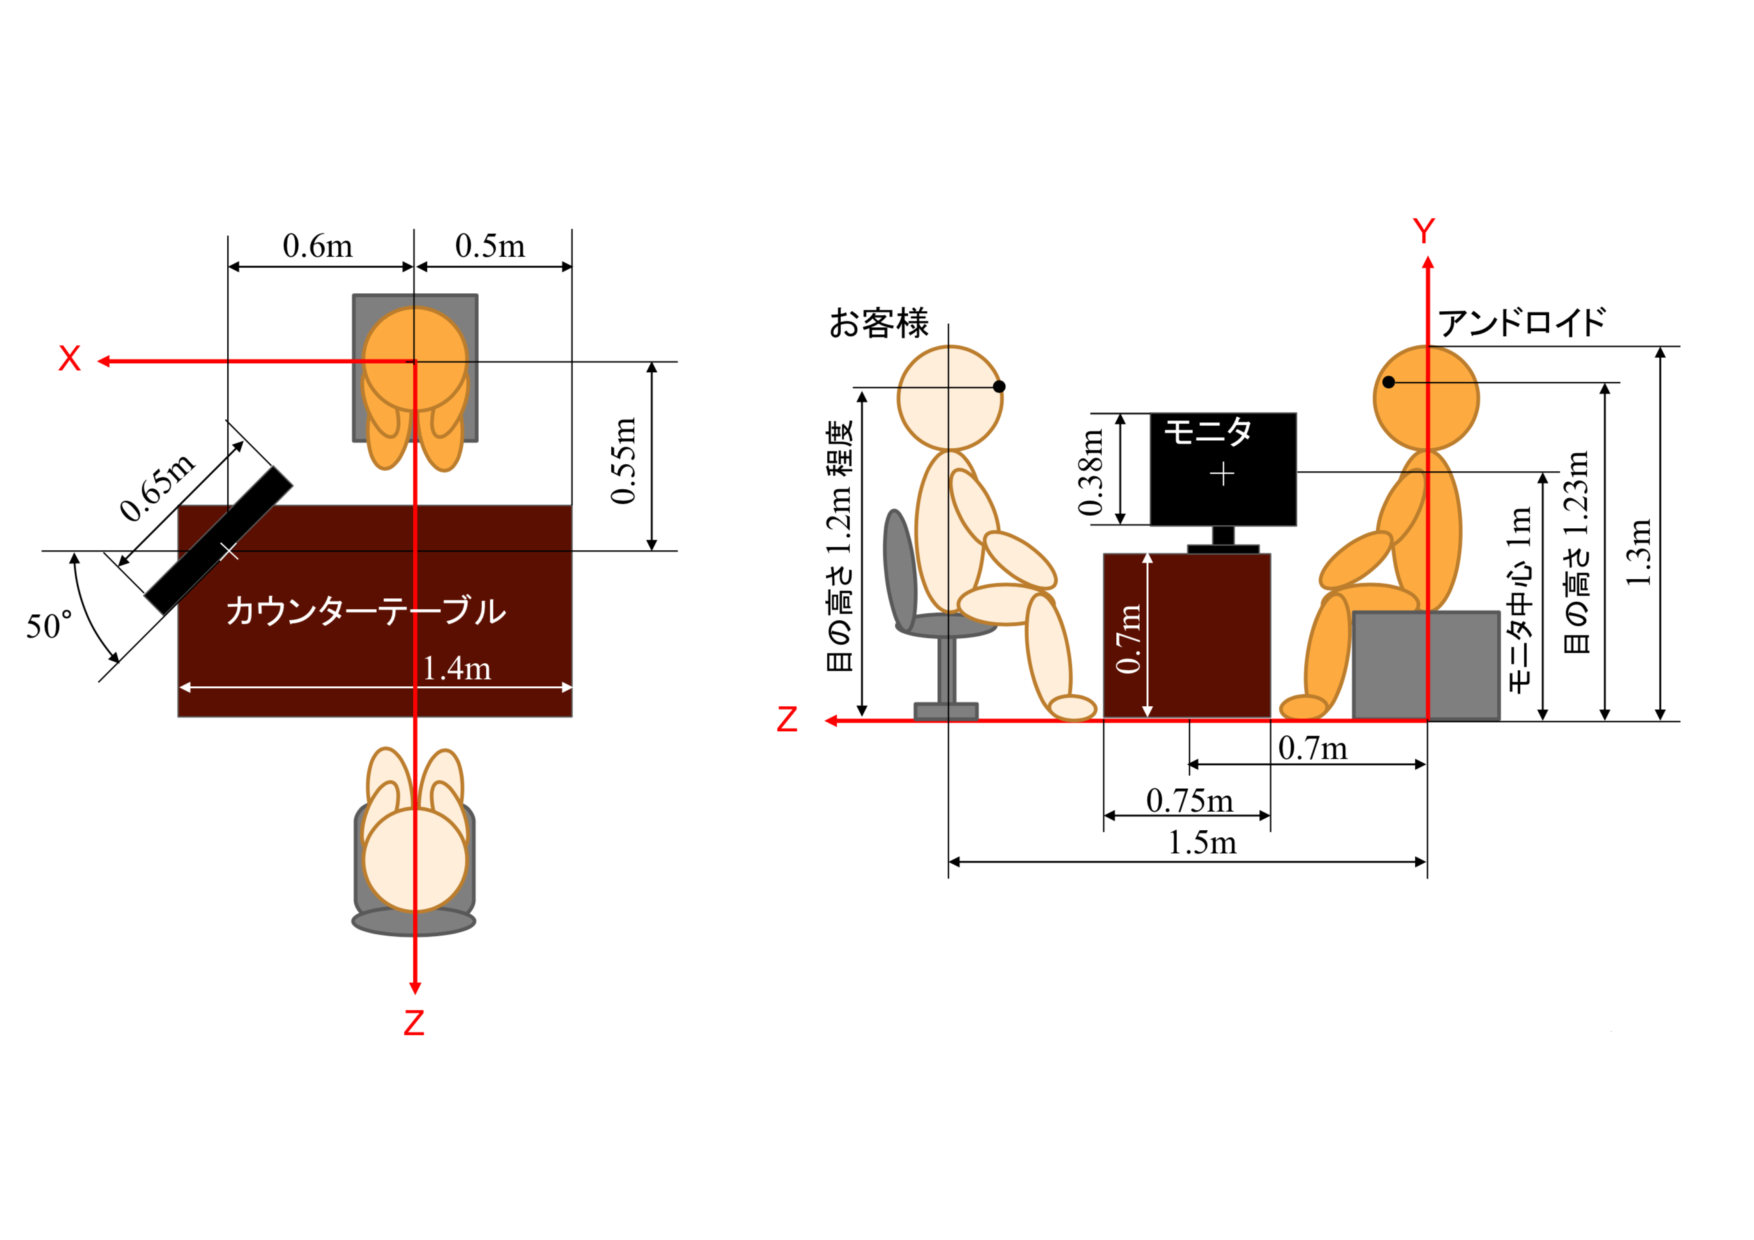
\includegraphics[scale=0.5,angle=270]{pic/robot_location.pdf}
        \caption{体験者とロボットの位置関係}
    \end{figure}
    \item ロボットに行わせてもよいこと
    \begin{itemize}
        \item 任意のタイミングで発話させること.
        \item 任意のタイミングで,視線,表情,頭部,上体等を動かすこと.
        \item 貸与された観光地情報を用いて説明すること.
        \item カウンター上のモニタに表示された観光地の写真について説明すること.
        \item 説明している観光地についての感想や意見を言うこと.ただし,開発指針として,本番で未知の観光地情報が与えられたとしても対応できるようにシステムを開発すること.
    \end{itemize}
    \item ロボットが対話中に使える情報
    \begin{itemize}
        \item 参加登録時に貸与される12箇所の観光地に関する観光案内情報.
        \item マイクとカメラで認識された,体験者の音声,表情,性別,年齢.
        \item モニタの位置(置いてある場所)の情報.
    \end{itemize}
    \item 観光地情報の扱い方
    \begin{itemize}
        \item 観光地情報データベースのレコードをプログラムで自由に操作して利用してよいものとする.
        \item 参加登録時に,本番で使用する観光地情報を渡すが,開発指針として,本番で未知の観光地情報が与えられたとしても対応できるようにシステムを開発すること.
    \end{itemize}
    \item 提案する観光地とお薦めの観光地
    \begin{itemize}
        \item 提案する観光地:対話開始前に,体験者は日本科学未来館近辺の6箇所,あるいはExpo City近辺の6箇所の観光地の中から,行ってみたいと思う観光地を2つ選ぶ.
        \item お薦めの観光地:2箇所の中からランダムに決定.
    \end{itemize}
    \item 対話タスクの開始・終了
    \begin{itemize}
        \item タスク開始前に,体験者から聞き出した2か所の観光地(A,B),その中からランダムに決定したお薦め観光地を参加者のプログラムに入力.
        \item テーブルのモニタ上に,観光地AとBの写真を並べて出力(Aが左,Bが右)モニタへの出力は主催者側で実行
        \item 体験者が椅子に着席した状態で,参加者のプログラムを開始.
        \item 対話開始から5分経過した時点,あるいは体験者がテーブル上のタブレットで観光地を決めたことを知らせてきた時点で,参加者のプログラムに対話終了.命令を入力し,対話タスクを終了.対話開始から5分経過しても対話中である場合は,体験者にタブレットで対話を終えるように伝える(主催者側が用意).
        \item 対話の始まりは,ロボットから話始めても,お客様の話始めを待っても,どちらでもよいとする.
        \item 対話終了後に,体験者にタブレットで観光地を選んでもらう.
    \end{itemize}
    \begin{figure}[th]
        \centering
        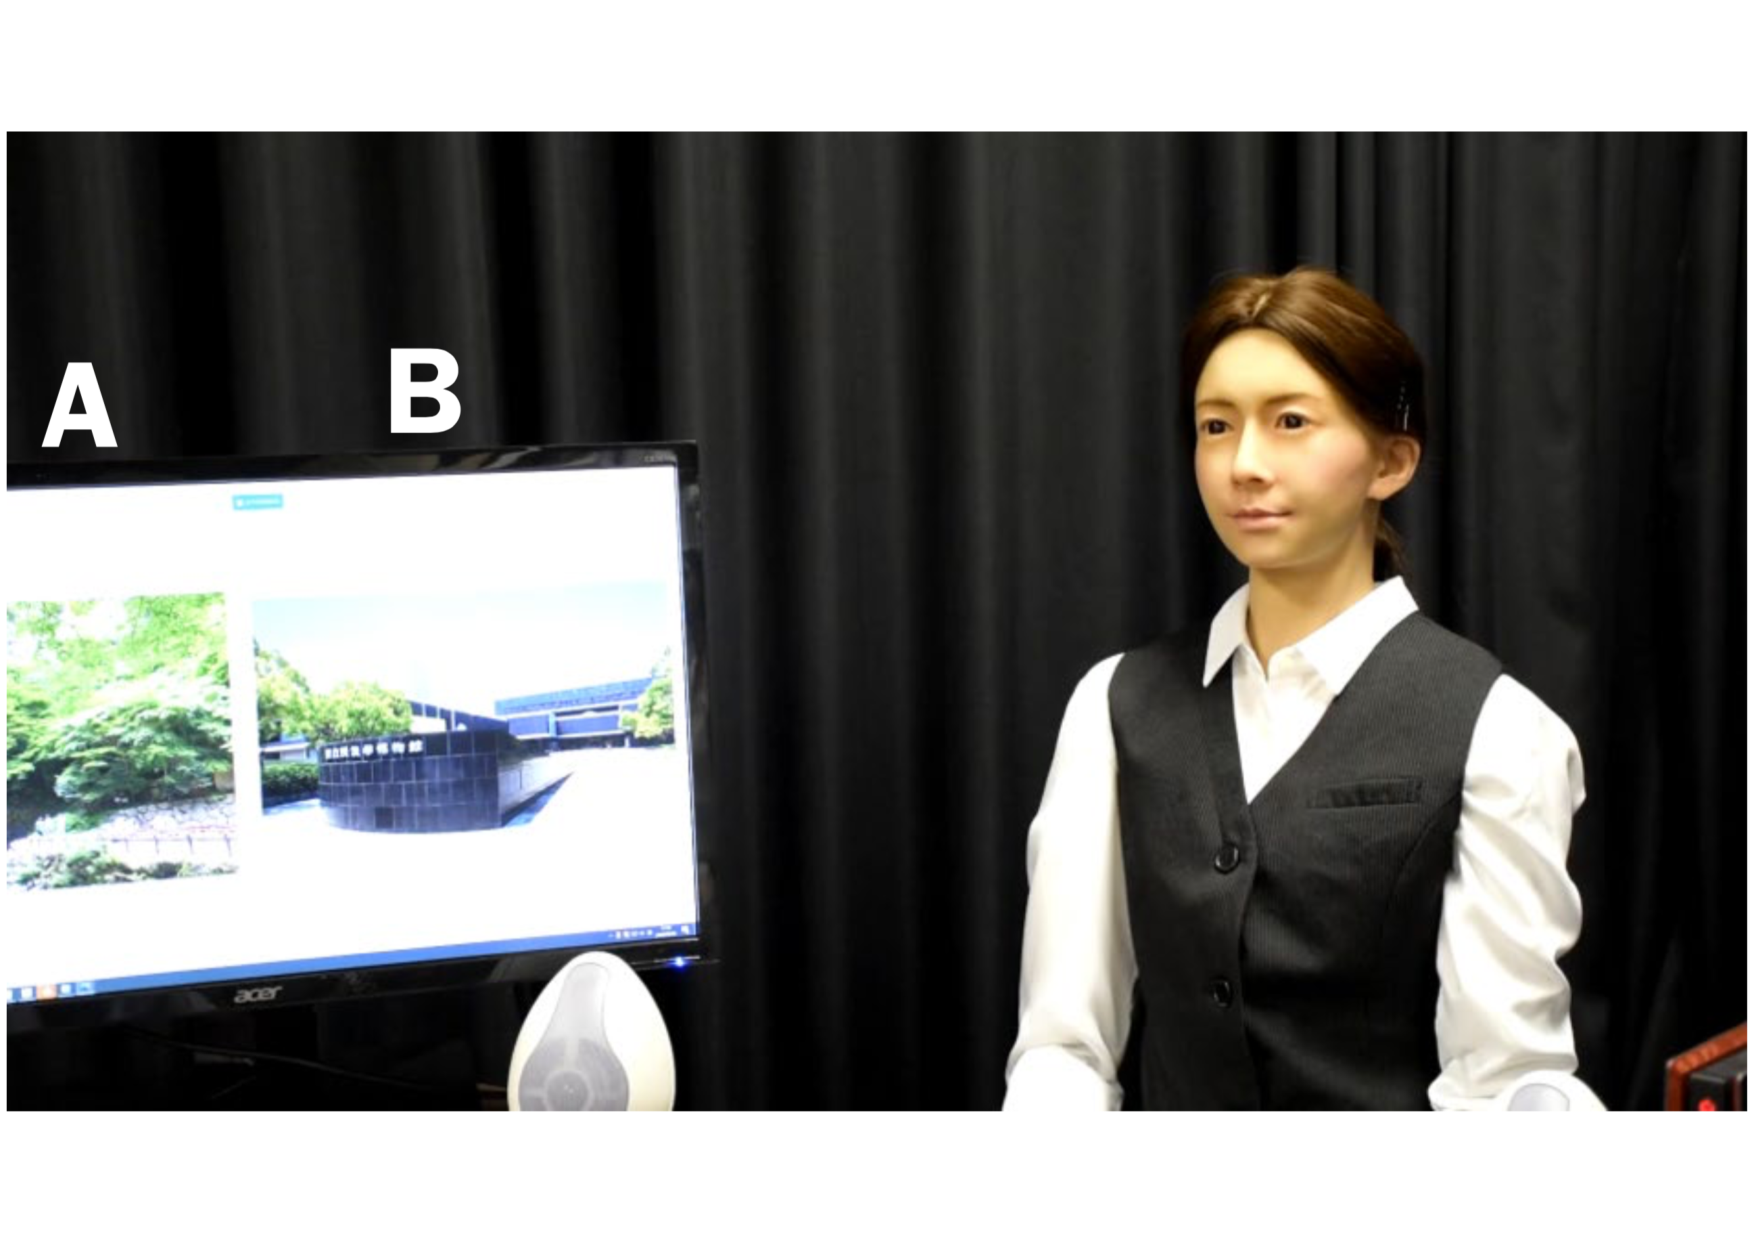
\includegraphics[scale=0.5,angle=270]{pic/AB_location.pdf}
        \caption{観光地の出力}
    \end{figure}
    \item ロボットに行わせてはいけないこと
    \begin{itemize}
        \item 対話以外の方法で,お薦めの観光地を体験者に選んでもらうこと(例:ロボットが,体験者に,お薦めの観光地を選んでもらったら賞品をあげるなどと言う).
    \end{itemize}
\end{enumerate}

\subsection{対話の評価手法}
下記の3つの観点から,システムの総合的な評価を行う.
\begin{itemize}
    \item 想定内の会話に対して構築通りの対話が実施できたか(動作確認)
    \item カウンターセールスとしてお薦めの観光地を選んでもらえたかどうか
    \item 体験者の満足度(対話後のアンケートによる評価)
\end{itemize}
まず動作確認では想定した会話に対して会話ロボットが想定した対話を実施できるかどうかについて評価する.
対話システムは反響や雑音がある対話環境で実施するため,音声認識,発話,対話管理システムが協調して
一貫した対話ができるかどうかを判定する.

次に上記の残り2つの観点についてアンケートを利用して評価する.
アンケート評価の評価項目は,下記の8つの観点である.1点の「そう思わない」7点の「そう思う」までの7段階で評価を行う.
\subsubsection{対話者の評価手法}
\begin{enumerate}
    \item 満足して遊びに行く観光地を選ぶことができましたか?(選択の満足度)
    \item 観光地の情報を十分に聞くことができましたか?(情報の十分さ)
    \item ロボットとは自然に対話できましたか? (対話の自然さ)
    \item ロボットの対応は適切でしたか?(対話の適切さ)
    \item ロボットとの対話に満足しましたか?(対話の満足度)
    \item ロボットの対応は好ましいものでしたか?(対応の好ましさ)
    \item 観光地を選ぶのにロボットから得られた情報を参考にしましたか?(情報の参考度)
\end{enumerate}

\subsubsection{ビデオ評価の評価手法}
COVID-19の影響で対話者が当初の想定より集まらず,チーム間での対話者の人数にばらつきがあるため,参加チームごと予選会場での対話を記録した映像を用いて,クラウドで追加の印象評価を実施する.評価項目は,下記の8つの観点である.1点の「そう思わない」7点の「そう思う」までの7段階で評価を行う.システムが正常に動かなかった場合などを評価から排除できるよう,各チームが3つの対話映像を選択し,それらを第三者に評価させる.
\begin{itemize}
    \item お客様とロボットの対話を第三者視点でどう思うかお答えください.
    \begin{enumerate}
        \item お客様はロボットから観光地の情報を十分に聞けていましたか?(情報の十分さ(客視点))
        \item お客様はロボットと自然に対話できていましたか?(対話の自然さ(客視点))
        \item お客様はロボットの対応を好ましく思っていましたか?(対応の好ましさ(客視点))
        \item お客様はロボットの対応に満足していましたか?(対応の満足度(客視点))
    \end{enumerate}
    \item あなたがこのロボットと対話したお客様だったらという視点でどう思うかお答えください.
    \begin{enumerate}
        \item あなたはロボットから観光地の情報を十分に聞けたと思いますか?(情報の十分さ(評価者視点))
        \item あなたはロボットと自然に対話できたと思いますか?(対話の自然さ(評価者視点))
        \item あなたはロボットの対応を好ましかったと思いますか?(対応の好ましさ(評価者視点))
        \item あなたはロボットの対応に満足したと思いますか?
        \item ロボットの話を聞いてあなたならどちらの観光地に行きたいと思いましたか?(どちらとも言えない場合は、強いて決めるとしたらどちらかで決めてください)
        \item このロボットは旅行代理店で実際にサービスできると思いますか?
    \end{enumerate}
\end{itemize}

\subsection{実験結果}
対話コンペティション全体として,大学8,高専1,企業2の11チームがコンペティションに参加した.各コンペティション参加チームはそれぞれ別日に「ららぽーとEXPOCITY」に来ている人を体験者として評価を行う.また,ビデオ評価では参加11チームのシステムと,実行委員の用意したベースラインを含めた12のシステムについて評価を行う.これらの評価と本論文のシステムとのアンケートによる比較は後ほど示す.

本研究で構築する対話システムのコンペティションは2021年8月23日,9月4日の2日間にかけて「ららぽーとEXPOCITY」で実施した.実験では午前中に会場に設定されているアンドロイドに対して接続テストを実施し,午後から体験者を募集して対話の実験データを獲得した.午前中に想定した会話に対する対話ロボットの動作確認を行った.また,実施した実験では2日間の合計で10代から50代の男女21人が体験者として参加して対話システムを評価した.
以下では各評価結果について記述する.

\subsection{想定した対話による動作確認実験}
対話システムをアンドロイドおよび出題をコントロールするタスク管理システムと接続して,動作を確認してから想定内の質問を実施した.
図\ref{fig:android1}にその様子を示す.図に示すように会話のスタート時にアンドロイドの姿勢を変化させて挨拶を実施している.
% 適当に入れて下さい.
%
\begin{figure}[h]
        \centering
        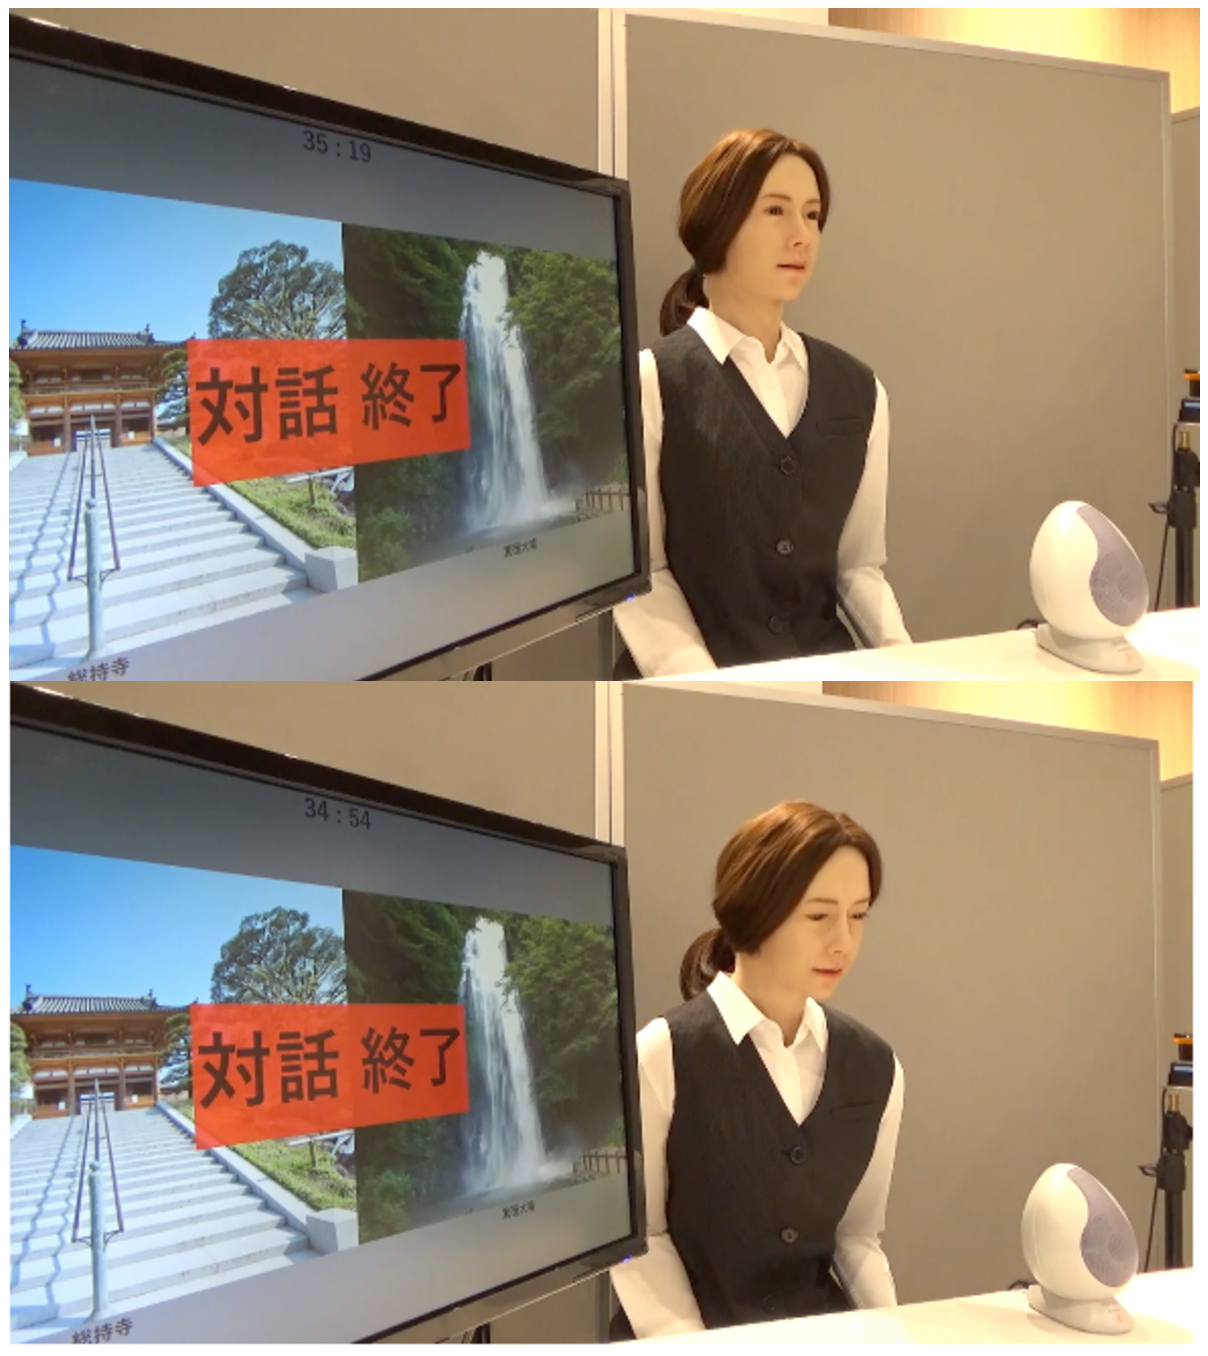
\includegraphics[scale=0.5]{pic/android1.eps}
        \label{fig:android1}
        \caption{対話スタート時に挨拶をするアンドロイド}
\end{figure}
体験者は対話システム構築者ではないが同研究室の教員である.体験者はどういう表現で動作しているか詳細を知らないが大きな会話の流れを
理解している状況で発話した.よって,体験者による発話はシステムを過度に意識することなく発話した.

以下に質問応答の結果とその様子を図で


\subsection{対話結果}
21

\subsection{アンケート評価の結果}
体験者21人のアンケート結果から表\ref{result_taiken}のような評価が得られ,ビデオ評価者50人のアンケート結果から表\ref{result_video}から以下のような評価が得られた.

\begin{table}[hbtp]
    \caption{体験者によるアンケート結果}
    \label{result_taiken}
    \centering
    \begin{tabular}{l|l|l|l|l|l|l|l}
    \hline
          & 選択の満足度 & 情報の十分さ & 対話の自然さ & 対話の適切さ & 対話の満足度 & 対応の好ましさ & 情報の参考度 \\ \hline
    評価の平均 & 4.05   & 4.10   & 3.14   & 3.62   & 3.86   & 4.00    & 4.24   \\ \hline
    順位    & 12     & 12     & 9      & 10     & 8      & 8       & 12     \\ \hline
    \end{tabular}
\end{table}

\begin{table}[hbtp]
    \caption{ビデオ評価によるアンケート結果}
    \label{result_video}
    \centering
    \begin{tabular}{llllll}
    \hline
    客観視点                    &                             &                             &                              &                             &      \\ \hline
    \multicolumn{1}{l|}{}   & \multicolumn{1}{l|}{情報の十分さ} & \multicolumn{1}{l|}{対話の自然さ} & \multicolumn{1}{l|}{対話の適切さ}  & 対話の満足度                      &      \\ \hline
    \multicolumn{1}{l|}{評価} & \multicolumn{1}{l|}{4.10}   & \multicolumn{1}{l|}{3.76}   & \multicolumn{1}{l|}{3.62}    & 3.86                        &      \\ \hline
    \multicolumn{1}{l|}{順位} & \multicolumn{1}{l|}{11}     & \multicolumn{1}{l|}{9}      & \multicolumn{1}{l|}{10}      & 8                           &      \\ \hline
    評価者視点                   &                             &                             &                              &                             &      \\ \hline
    \multicolumn{1}{l|}{}   & \multicolumn{1}{l|}{情報の十分さ} & \multicolumn{1}{l|}{対話の自然さ} & \multicolumn{1}{l|}{対話の好ましさ} & \multicolumn{1}{l|}{対話の満足度} & 実用性  \\ \hline
    \multicolumn{1}{l|}{評価} & \multicolumn{1}{l|}{3.96}   & \multicolumn{1}{l|}{3.90}   & \multicolumn{1}{l|}{3.81}    & \multicolumn{1}{l|}{3.51}   & 3.74 \\ \hline
    \multicolumn{1}{l|}{順位} & \multicolumn{1}{l|}{10}     & \multicolumn{1}{l|}{11}     & \multicolumn{1}{l|}{11}      & \multicolumn{1}{l|}{11}     & 11   \\ \hline
    \end{tabular}
\end{table}

\section{考察}
\label{考察}
\subsection{対話ロボットに関する考察}

\subsection{対話制御に関する考察}

\section{まとめ}
\label{まとめ}

\section*{謝辞}
\addcontentsline{toc}{section}{謝辞}
本研究を進めるに当たり,指導して下さいました竹内孔一先生に心より感謝致します.また,議論に参加して下さいました竹内研究室の諸氏に心より感謝致します.

\addcontentsline{toc}{section}{使用したツール}
\section*{使用したツール}
\begin{itemize}
\item 工藤拓.形態素解析 MeCab.http://taku910.github.io/mecab/
\item Google.音声文字変換 Speech-to-Text.https://cloud.google.com/speech-to-text/
\item Amazon.テキスト読み上げ Amazon Polly.https://aws.amazon.com/jp/polly/
\item Oculus.口形状生成.https://developer.oculus.com/downloads/package/oculus-lipsync-unity/
\item Google.Google Maps API.https://developers.google.com/maps/
\end{itemize}


\addcontentsline{toc}{section}{参考文献}
\nocite{*}
\bibliographystyle{junsrt}


\bibliography{biblio}

\end{document}
